\documentclass{article}
\usepackage{xcolor}
\usepackage{amsmath}
\usepackage{graphicx}
\usepackage{xcolor}
%
\definecolor{awesomeblue}{RGB}{0,74,127}
\definecolor{awesomebrown}{RGB}{191,99,40}
\definecolor{awesomeskyblue}{RGB}{0,148,255}
\definecolor{awesomeyellow}{RGB}{236,192,27}
\definecolor{awesomered}{RGB}{228,36,51}
\definecolor{awesomeorange}{RGB}{243,119,56}
\definecolor{awesomewinered}{RGB}{168,34,110}
\definecolor{boringgreen}{RGB}{130,179,102}
\definecolor{boringblue}{RGB}{108,142,191}
\definecolor{boringred}{RGB}{184,84,80}
%
% TITLE
\title{Decentral Card Network}
%
% AUTHORS
\author{Patrick Wieth}
%
% CONTACT INFORMATION
%\email{second.author@example.com}
%
\begin{document}
\maketitle
%
\begin{abstract}
In this paper the concept of a decentralized trading card game is introduced. This class of games has the specific feature that game assets have a value outside of the game. This means players are not only accumulating ressources ingame but also between games. Magic the Gathering\cite{mtg} invented this revolutionary game concept and later it was adapted on PC and online. The most popular digital trading card game is Hearthstone\cite{Hearthstone} at the moment. Unfortunately this game strips off a crucial part of such games, namely the trading with other humans. Here we want to present a concept that goes even further and does not only implement card ownership on a blockchain but also creation of new cards as well. Thus not only the design of decks and combination of cards is a creative process being done by players, but also the design of the game itself. 
\end{abstract}
%
\section{Introduction}
%
It is quite surprising that Magic has remained the most popular trading card game offline, whereas it has not succeeded online. There might be several reasons why Magic was not really successful online and Hearthstone made it. An obvious reason might be that Magic is as expensive playing online as playing it with real cards in the case of Magic Online or being a closed space game, with a limited card pool and no real interaction with other card collectors in various examples. Furthermore playing Magic is quite clunky and turns of opponents might take long, which is less annoying when playing face to face. In contrast Hearthstone offers a much more convenient experience, is free to play and strips off many aspects of magic, which are sources of complexity. This leaves lovers of Magic's deep strategy dissatisfied and of course offers less card variance. But the biggest disappointment from Hearthstone might be that the players are not the owners of the cards. An important property of trading card games is that you own the cards, you are able to sell them to other players, so collecting them makes actual sense. In Hearthstone you don't own the cards. You have an account that let's you play with cards you have acquired within the game, you have not acquired these cards in the real world. Accordingly you cannot sell these cards to other humans. Furthermore if Blizzard's server goes offline, for instance if the company is sold or goes bankrupt, then your cards are gone as well. The same applies to Magic Online, but at least there one would expect that Wizards of the Coast might offer you to print your cards and being sent to you, if they shut down their servers. However, you are dependent on a centralized service, giving life to your card base. It is obvious that blockchain technology is a solution for this problem, offering real ownage (since this is a paper, puns are not officially intended). 
%
\section{Decentralizing a trading card game}
%
Given these aspects it is not surprising blockchain based trading card games have already popped up. Given the other aspect that currently just appending blockchain/crypto to a products name leads to higher media coverage, it is even less surprising that trading card games are built on blockchains. Thinking further about these games it strikes also, that a key component of success is the constant stream of new game elements. To keep these games interesting it seems to be necessary to introduce new cards on a regular basis. There have been a lot of competitors to Magic and they were quite successful in the beginning and have drawn a lot of attention, but whenever the stream of new cards slowed down, the games lost popularity. Therefore a company creating such a game necessarily needs to produce new cards to keep the game alive. Thinking in the approaches blockchain technology offers, one should not only consider to give real ownage of assets to users but also think about reorganizing corporate structures. In Magic not only famous artists exist, whose designs are loved by the community, but also community members exist who alter the design of cards and these altered designs are loved as well. This leads to the idea to decentralize the process of card design. Why have a company that hires artists and organizes card design, if the blockchain technology enables to have not only owners of card instances but also authors of cards. The authors of cards decide how many will be printed and profit directly from selling the cards. In this sense the cards of decentralized card game are not only owned by the community but also made by the community. Thus we call it Decentral Card Network now, since it is not just a game, but rather a network. Of course this spawns a lot of concerns and questions, the most important ones might be:
%
\begin{itemize}
	\item How will the creation of ridiculously overpowered cards be prevented?
	\item How is the quality of the artwork ensured?
	\item What if authors use copyrighted imagery or abusive pictures?
	\item Even if creators try to balance their cards, how will all card creators be synchronized to a common power level of cards?
	\item Won't card creators just print insane amounts of their own card and sell like crazy?
	\item What do you want to do against trolls, putting Hide the pain Harold, funny cat images or sad frogs on cards?
\end{itemize}
%
Of course there are even more questions, that might be asked, but most of the questions are variations of the main question "How do you make authors not ruin the game?". It seems simplistic to reduce all these questions to such a single question, but there might be only two approaches necessary to answer all of them. Let's pick out a very specific question "Why would anybody put much effort in this and create a card?" - the answer is quite simple, because it is economically favorable to do so. Creating cards gives you ingame credits and if the demand is high enough these credits can be traded for real money on cryptocurrency exchanges just like other crypto assets. Therefore it is just a matter of tuning the correct parameters of the cryptoeconomics of Decentral Card Network. This answer can be applied to other questions as well, such as "how to make authors create fair cards" or "Won't authors just print insane amounts of their card?". Of course there are situations where economical incentives won't cut it. The obvious one is "What if someone wants to break the game?", then the game must not allow such a thing to happen. We assume the majority of users to be acting rational. We don't assume everyone behaves rational only the majority. This means economic incentives work for this majority. We can get to fair card creation by punishing creators for unfair creations and reward players for pointing out broken cards. To be more precise, there will be two mechanisms, one acting on card creation and the other one on all existent cards. First after a card \textit{draft} has been created, it goes to the \textit{council}, which consists of 5 active players, who have to lock some credits to participate in the council. They are allowed to vote on the card draft to pass the council, demand a revision with a list of critique points or deny the card draft. The vote is not only a vote, it is also a bet. After all voters have committed their vote, the majority vote gets elected. If the draft is denied, the minority of positive voters lose their funds for the benefit of the deniers. If a revision is requested, the card creator has time to rework the card and then the vote happens again. If the majority confirms the card it becomes a \textit{prototype} card. A prototype is on trial for the next couple of weeks and all council memebers as well as the creator get one prototype copy. They are now eligible to play with the prototype and their opponents are incentivized to mark the card. Marking a card is the second mechanism of the two mentioned previously. Whenever a game is finished both players are allowed to mark cards from the decklist of their opponents. Cards can be marked as overpowered (\textit{OP}), underpowered (\textit{UP}), \textit{fair}, copywright violating (\textit{cv}) and \textit{abusive}. This is possible for prototype as well as for \textit{permanent} cards, it has different implications though. For cards on trial, prototypes, it is necessary to be voted as fair by some players to become a permanent card, in addition the OP, cv and abusive votes must be very low in comparison to the average rate of negative marks. If the card is either marked too often negative or does not receive enough fair or UP marks, the prototype is revoked. In this case the deniers from the council win the bet and the approvers lose their locked funds. In the other case, where enough fair or UP marks are set, the deniers lose their locked funds and the approvers win the bet. Only left is the explanation of the effect of card marks for permanent cards. In this case cards are rebalanced, meaning their properties are nerfed if they are statistically often marked as OP and buffed if they are often marked as UP. In the case of many copyright violation votes, the copyright of the artwork is checked by the stakeholders of Decentral Card Network and transferred if necessary. In the case of abusive cards, either the image or the information text of a card are inappropriate, such as child pornography or racism etc, the card will be removed if the stakeholders approve the vote. This is also an answer to the question what if authors use abusive pictures. In contrast regarding funny cat images or sad frags, we want to state here, that we desire to have pictures of old men hiding their pain in this game.
%
\section{Emerging game balance}
%
As already explained the aim of the these mechanisms is to balance the cards so that the game is playable. The balancing happens through nerfs and buffs on the properties of the cards. Specifically this means the cost of a card is adjusted as well as the speed. We will explain the game mechanics later, though some readers might guess what these properties mean. After a card has passed the council, it has a base cost of ressources and a base speed, if a card is nerfed for the first time, the cost is increased at least so much that one of the ressources it costs increases by one integer, the second time it gets nerfed, the speed is increased by 1 (lower values mean faster). The next time the cost is increased again, then the speed and so on. Buffing works the same, except that the cost is lowered and the speed as well. If cost arrives at 0 or speed at 1 then only the other value is buffed subsequently. If both arrive at the minimum value the card cannot be buffed anymore. At first glance it seems that this is sufficient to prevent cards from being too strong, since their cost will be nerfed as long as they are too strong. But knowing such games well, one must consider that it is often possible to circumvent the cost of a card with other cards. If the other card does exactly that, there is no problem, since then the other card is the one to nerf. But it might also be possible to play a card when it is discarded to the dust pile or it can even be played from the dust pile (graveyard or discard pile). So if a card offers to be played from the dust pile, it is possible to discard it with some other card or effect and then play it. Even if the community realizes that the card is overpowered and reacts by voting for a nerf, the nerf has no effect, since it increases the casting cost of the card and reduces the speed. The casting cost is not relevant, since the card is not played for its casting cost and the speed might not be relevant, if the card can be played very early at no cost. To solve this issue one can think about not only buffing or nerfing the cost and speed of a card but also its effects. However this solution creates more problems and is not advisable. For example a card can have the effect that opponents cannot play spells as long as the card is in the graveyard. This effect is complicated to nerf in an automated way and it is very strong. If such a card happens to pass the council, it cannot be nerfed, since any discard effect effectively activates the card and gives you a very strong effect circumventing all costs. We conclude at this point that some things cannot be balanced and the game mechanic must prevent unbalanceable cards. A solution in this regard is to deny card effects from cards in the dust pile. The only exception might be effects that have the cards cost as activation cost for the effect usable in the dust pile. \newline
Therefore we realize that we must secure by game mechanics that all cards can be balanced and then it is possible to have a community driven global game balance. We will explain how to drive players to do favorable things later in the token economics section. For now it is sufficient to understand the basic concept.
%
\section{Game Mechanics}
%
The core of a trading card game is a set of cards, usually called a deck. In contrast to most other card games the set of cards is not the same for every game played. The players bring their own set of cards to a game and play with or against others who have done the same. Cards can be picked from a lot of cards, which are continuously released in sets or editions. As already outlined a constant stream of new cards is very important. We don't want to change this part but we want to change a lot of other parts. The most important aim of the game mechanics is to provide a convenient game experience together with a deep complexity. We believe that these two properties do not exclude each other necessarily. For Magic the Gathering the frustration mostly comes from watching long phases of planning a turn as well as responses within a turn, which often stop the game flow. Even if a player has planned his turn during the turn of the opponent, it happens often that a newly drawn card provokes new planning. In addition while the opponent's turn is ongoing and you plan your next turn, you have to wait what the opponent plays, before you can make good decisions. These phases of waiting seem to be the biggest source of game flow disruption. Our main goal is to avoid game flow disruption without sacrificing complexity. In Hearthstone the problem was resolved by giving up a lot of interesting complexity regarding game mechanics. Taking away the possibility to do things on opponents turns allows for time limits on turns and speeds up the game. In addition the cards are much simpler in most cases as well. Our solution is to give up turns. We want to stick to a turn-based game, but all players play simultaneously. We will refer to two players subsequently for brevity, but this works for multiplayer nonetheless. Giving up turns but not giving up turn-based strategy means that we arrive at micro-turns, which we call \textit{ticks}. We also don't give up the concept of a stack. This means spells and abilities do not resolve instantaneously but rather go to a stack where they resolve. In Magic the stack is organized in LiFo, last-in first-out, so whenever you have a response, you can play it and it resolves before the thing you respond to. In Magic the game designers differentiate between cards that can respond to other cards and those that can only be played when nothing is on the stack. These two card speeds are also accompanied by a third speed which can respond but is so fast, nothing can respond to it. We want to further improve this concept of card speed by giving cards an integer speed. Cards can then have a speed from 1 to ludicrous high numbers. The stack is then not organized in a LiFo manner but rather a FiFo with ticks. So if two cards are played at the same time, the one with a lower speed integer resolves first. Since turns are abolished, speed also determines how long it takes a card to be usable again. In Magic cards are tapped when used and untap at the beginning of a turn. In Decentral Card Network turns do not exist. Whenever an activated ability of a card is used, it goes to the stack and it takes time depending on card speed until it resolves. The production of ressources happens in the same manner, but are a periodic ability. Periodic abilities are passive abilities, which put their effect on the stack again, whenever the old effect is resolved or countered. Before we give an overview of all ability types, we will finish the core mechanics first. In Decentral Card Network there is a Headquarter for each deck. The headquarter or \textit{HQ} is in play when the game starts and usually has a production ability, that creates some ressources, has a way to draw cards, has attack/health and speed. For example Magic's rules transferred to a HQ, it has 0 attack, 20 health and draws a card peridically. In Decentral Card Network lands do not exist and continuously increasing mana crystals also don't exist. In contrast all cards can possibly produce ressources and the HQ is a source of ressources players have right from the start. Therefore the concept of designing how a deck "ramps" is not removed like in Hearthstone and a concept like lands is omitted, because it is either a source of disrupted game flow when no lands are drawn or is a rule of limited ressource grow per turn that can be worked around easily. Precisely in Magic this means you cannot only design your deck to have consistent land drops but also increase the mana curve by using spells that pull additional lands from the deck, having creatures, artifacts and enchantments, which produce mana as well as spells that give a short term boost to mana. We think it is desirable to give the players control over their income curve, since this is an interesting strategic element of most strategy games. But we don't want to have a special card type like lands, we rather have a HQ card in the game at the beginning, which removes a lot of cases where a game is pointless, because one player does not draw enough lands, which is a big source of game flow disruption. Furthermore, we don't deplete the resource pool at a given time, so even if the first wave of income from the HQ is not sufficient to play a card, the second or third wave should accumulate enough ressources. In addition all permanent cards can produce ressources and single effect cards can give short term boosts to ressources. At first glance this seems like the income grows exponentially rather than linear, which is true as long as you ignore card disadvantage as well as the necessity to interact with your opponent. In fact we use the term ressources here for things like mana, lumber, or food, but from a game design point of view, cards in your hand, cards in play and your life are ressources. Life in Magic or Hearthstone correspond to health of the HQ in Decentral Card Network. Understanding all these points, the HQ serves several purposes. Let's make a list:
%
\begin{itemize}
	\item Defines how cards are drawn
	\item First source of ressource income
	\item Defines how much life a player has
	\item Brings additional intrinsic mechanics to a deck
	\item Possibly defines additional ways to win or lose a game for a deck
\end{itemize} 
%
The first three points have been explained already, the last two are consequences of HQs being quite similar to commanders in Magic's format EDH/commander. This format has emerged in Magic only after many years and brings additional complexity to the game, because a specific creature can be picked to be available at all times, thus allowing to build a deck around its unique abilities. We think this is very desirable. Especially in a game, where cards are rebalanced forever, so that there won't be absurd and undesirable interactions or even single cards. Furthermore the HQs give the power to design format defining cards to the players. We think how a game is played and how tournaments are arranged should not be dictated by the game producers, because it does not take long until the community as a whole has a better understanding how the game should be played than the initial designers. It is desirable to have some HQs typical for competitive 1on1 games as well as others for more casual multiplayer rounds. It might also be interesting to have tournaments, which only allow for a small set of HQs, so that the meta-game becomes easily understandable. This is why we prefer solutions with cards, that can be designed and balanced by the players, over some pre-defined formats or specific game rules like draw a card every 5 ticks etc.
%
\section{Token Economics}
%
It is obvious, that getting the flow of cards and currency right is the most important thing for a project like Decentral Card Network. Having too many cards dropped on the player's heads is boring as well as incredible slow progress is frustrating. So finding the balance is crucial. Furthermore not only the microcosmos of a player's motivation vs. frustration needs to be balanced, the whole sphere of cards that are going to be mass produced needs to be in balance as well. In this section we will outline the economics starting from the perspective of a new player in chronological order. That way we can also give insight how a player is confronted with the game over time and what choices are available.
%
\subsection{Account creation and game reporting}
%
A new player who creates an account gets a whole set of base cards and starts with 1 credit, the in-game currency. The base cards consist of two base HQs, thus allowing two different deck types and also enough cards to play both of these decks. The player may shift cards between the two decks or start a game. Starting a game means the player has to lock in a deck he wants to play with and is matched with another player. The blockchain keeps record of the locked decks and matched players. Now both players can play against each other, in the bootstrapping phase of Decentral Card Network, there won't be a game client, so they have to meet in another client such as Magic Workstation\cite{MWS}, untap.in\cite{untapin} or similar available applications. Later there might be several game clients or just a single one, ideally organizing the game in a blockchain as well, but not on the main chain, which keeps track of card ownership. After the game has finished, both players have to report on the game. Only if a playe has reported the game result, another game can be started. A game report is basically a transaction to the blockchain, which states how the game result is or why it hasn't started. If a player realizes that the game with the matched opponed won't start, the following reports are possible:
%
\begin{itemize}
	\item 1. Communication with opponent wasn't possible or he didn't want to play, maybe it's a bot.
	\item 2. I had no interest in playing the game or weren't able to play it anymore.
	\item 3. We weren't able to connect to each other in-game or we both didn't want to play.
	\item 4. I have no clue whatsoever.
\end{itemize}
%
The blockchain evaluates both answers and increases the troll\_counter of the players according to following table, where a minus is an increase of the troll\_counter, the color is the player and the number is the reported reason:
%
\begin{center}
	\begin{tabular}{ c | c | c | c | c }
		& \textcolor{blue}{1} & \textcolor{blue}{2} & \textcolor{blue}{3} & \textcolor{blue}{4} \\ \hline
		$\textcolor{red}{1}$ & $\textcolor{red}{{}_{---}} \textcolor{blue}{{}^{---}} $ & $\textcolor{blue}{-} $ & $\textcolor{red}{{}_{---}} \textcolor{blue}{{}^{---}}$ & $\textcolor{blue}{--}$ \\ \hline
		$\textcolor{red}{2}$ & $\textcolor{red}{-}$ &  &  & $\textcolor{red}{-}$ \\ \hline
		$\textcolor{red}{3}$ & $\textcolor{red}{{}_{---}} \textcolor{blue}{{}^{---}}$ &  &  & $ \textcolor{blue}{-}$ \\ \hline
		$\textcolor{red}{4}$ &  $\textcolor{red}{{--}}$  &  $\textcolor{blue}{-}$  & $\textcolor{red}{{-}}$ & $\textcolor{red}{{}_-} \textcolor{blue}{{}^-}$ \\ 
	\end{tabular}
\end{center}
%
The troll\_counter is to determine which players are either bots, keep crashing games or accuse others of crashing games even though they are the resason for it. If the troll counter exceeds 10 and exceeds the number of games played, then a player gets a ban for 24 hours. If it exceeds 100 and the number of games played succesfully, the account gets banned. If a player does not report on a game for 24 hours, then it is automatically reported from his side as option 4. The design of the troll table is mostly done so that players are punished for giving impossible answers the strongest and being punished not at all if they were cooperative and honest. Only small punishment is given if the player messed up but is honest about it. At first glance it might seem strange, that if two players both report each other as non-communicative, both get a big punishment. Assuming one player is honest and the other wants to troll him, he gets the biggest punishment, even though he was honest, just the other trolled him. However for the blockchain it cannot be determined who is the honest one of both, it would need a third human to see chat and communication attempts to decide, who is the real troll. Still this concept works, since someone who is honest will only encounter such a troll once in a while, where in contrast  the troll always encounters himself after each unsuccessful game. So if he keeps trolling, he accumulates a lot of troll increments until he gets finally banned.
%
\newline \newline
%
Let's return to the more fun part, a game that actually finishes. Again players can report here. The options are:
%
\begin{itemize}
	\item 1. I won.
	\item 2. I lost.
	\item 3. It's a draw.
	\item 4. I left the game.
	\item 5. The other left the game.
\end{itemize}
%
Depending on both player's reports the following table explains what happens:
%
\begin{center}
	\begin{tabular}{ c | c | c | c | c | c}
		 & \textcolor{blue}{1} & \textcolor{blue}{2} & \textcolor{blue}{3} & \textcolor{blue}{4} & \textcolor{blue}{5} \\ \hline
		$\textcolor{red}{1}$ & $\textcolor{red}{{}_-} \textcolor{blue}{{}^-} $ & $\textcolor{red}{++} $ & $\textcolor{red}{{}_-} \textcolor{blue}{{}^-}$ & $\textcolor{red}{{}_+} \textcolor{blue}{{}^-}$ & $\textcolor{red}{{}_-} \textcolor{blue}{{}^-}$ \\ \hline
		$\textcolor{red}{2}$ & $\textcolor{blue}{++}$ & $\textcolor{red}{{}_+} \textcolor{blue}{{}^+}$  & $\textcolor{red}{{}_+} \textcolor{blue}{{}^+}$ & $\textcolor{blue}{-}$ & $\textcolor{blue}{+}$ \\ \hline
		$\textcolor{red}{3}$ & $\textcolor{red}{{}_-} \textcolor{blue}{{}^-}$ & $\textcolor{red}{{}_+} \textcolor{blue}{{}^+}$ & $\textcolor{red}{{}_+} \textcolor{blue}{{}^+}$ & $\textcolor{red}{{}_+} \textcolor{blue}{{}^-}$ & $\textcolor{red}{{}_-} \textcolor{blue}{{}^-}$ \\ \hline
		$\textcolor{red}{4}$ &  $\textcolor{red}{{}_-} \textcolor{blue}{{}^+}$  &  $\textcolor{red}{{}_-}$  & $\textcolor{red}{{}_-} \textcolor{blue}{{}^+}$ & $\textcolor{red}{{}_-} \textcolor{blue}{{}^-}$ & $\textcolor{red}{{}_{-}} \textcolor{blue}{{}^{++}}$ \\ \hline
		$\textcolor{red}{5}$ & $\textcolor{red}{{}_-} \textcolor{blue}{{}^-}$ & $\textcolor{red}{{}_+} $ & $\textcolor{red}{{}_-} \textcolor{blue}{{}^-}$ & $\textcolor{red}{{}_{++}} \textcolor{blue}{{}^-}$ & $\textcolor{red}{{}_{--}} \textcolor{blue}{{}^{--}}$ \\
	\end{tabular}
\end{center}
%
This table is a bit more complicated as the previous one. It does not only increase the troll\_counter for all entries with a minus sign, it also gives credits proportional to plus signs. The concept is the same, if player's are honest, they are not punished and the winner of the game gets 2 credits. If a draw happened both get 1 credit and if one player left, the troll\_counter is increased. If a player reports a game result and the other reports a game that didn't come into existence, then the report of the game result is treated as (1) Communiaction with opponent wasn't possible or he didn't want to play, maybe it's a bot. 
%
\subsection{Reporting of cards}
%
If a game was finished, both players may review the decklist of their opponents. This means they can mark cards as either overpowered (OP), underpowered (UP), fair enough (FE) or inappropriate (IA). A card might have a pool of evaluation credits, which gives players marking the card credits until it is empty. For the player this means, if you see cards in the opponents decklist that have a non-empty pool, it makes a lot of sense to mark the cards. For every mark you give, you are awarded with 1 credit. You can also mark cards with a non-empty pool, but this costs you 1 credit, except for the winner, who has a single free evaluation. Typically cards with a non-empty pool are new cards, which need to be evaluated for passing the trial phase. But you can also spend your credits if you feel like your opponent is playing only unfair cards. One might ask, what the fair enough mark is for, since why would you report a fair care? This is important for said new cards, that give you 1 credit, regardless how you evaluate it. If the card is fair, you might want to say exactly that and still get your credit. For cards that are not on trial, this might seem useless, but it offers players to pose a counterbalance on cards that are deemed to be nerfed soon. Also players can donate their credits to the evaluation pool of a card, incentivizing others to vote on it. A typical scenario might be, that a reddit shitstorm has started against a card, calling players to vote it OP and donate their credits to the pool of that card. For the literate redditor who is not convinced by the hysteria of the masses, he can mark fair enough as well.
%
\subsection{Card creation}
%
After the game, the player might play another game or spend his earned credits to buy booster packs or buy specific cards from others. Buying a booster pack is the typical way to acquire new cards in this type of games. Boosters can only be bought from active card collections and a purchase yields 1 rare card, 3 uncommon and 9 common cards. The price for a booster will most likely be fixed, for example to 15 credits. But it might also be possible to leave it open to the designers of the card collection. In that case they will find a price, where the product of price and units sold reaches a maximum. The question is, if the found price is the same as the price where players get enough new cards to be motivated and not too many to be spoiled.
%
\newline \newline
%
After a player has traded with others, bought boosters, played a lot of games and maybe participated in tournaments, she thinks it is time to create a new card of her own. Card creation schematics are auctioned and the price depends on demand. Once in an hour a schematic is auctioned. The paid credits from the auction go to the winner's pool, from where the 1 credit for a won game is subtracted. Now our player has acquired such a schematic and wants to activate it, which means a card has to be designed and additional fees must be paid. These fees depend on the card type and rarity. A common costs 25 credits, an uncommon 50 credits, a rare 100 credits and a HQ 200 credits. This is a good point to note that rarity shall not imply strength of a card. In most trading card games, rare cards are also stronger cards, this is not intended here. But rare cards have complexer rules. A common might have a complexity of 5, an uncommon 10 and a rare 20. A headquarter has a maximum complexity of 30. The concept of complexity is quite simple, every building block of rules in a card increases it by 1. A common card for example, might be able to attack and to block attackers, giving it a complexity of 2, adding a speed modifier of -2 to the block ability increases its complexity to 3, giving the card "produce 1 lumber" as well as "regeneration 2" also increas by 1 each. In addition three integer numbers have to be chosen for attack, health and speed of the card as well. These values have no impact on complexity and are mandatory for objects and headquarters, for action cards only speed is mandatory. Some single abilities might have a high complexity, for example "whenever a creature dies, create a 1/1-5 skeleton creature with attack and block abilities. 1/1-5 means it has 1 attack, 1 health and speed 5. The creature brings a complexity of 3 alone, the whenever trigger brings an additional complexity as well as the "a creature dies" event. This means the ability would already fill the whole complexity available on a common card. The last mandatory spec of a card is the cost of a card. After a valid card has been designed, it can be submitted to the blockchain by paying the fee. This fee is in fact not really a fee but a collateral. If the card is created successfully, it goes to the council. The council consists of 5 players, who have also locked in a collateral of 20 credits each. They can vote on the card now, with 4 options
%
\begin{itemize}
	\item 1. The card is overpowered.
	\item 2. The card is underpowered.
	\item 3. The card is inappropriate. 
	\item 4. The card is fair enough.
\end{itemize}
%
Only option 3 needs explanation, this is mostly to prevent names and images which are inappropriate and a reason can also be given. If the card receives less than 3 fair enough votes, it goes into revision, the card author can upload a new version within 24 hours. The council is held again and if less than 3 fair enough votes are given, the card creation is rejected. In this case the fee paid by the card's creator is distributed among the council members who voted no. The same applies for the fees of the positive voters. But a maximum of 40 credits is given back, so doubling the investment is possible here. If credits remain, they go to the public pool. If there are enough positive votes, the council approves the card. Every council member gets a copy of the card and thus can play with the card. This starts the next phase, the Trial, which lasts for 2 weeks. At the end of the trial the card is finally approved or rejected. The cards trial score is evaluated as follows:
%
\begin{equation}%
s = \frac{m_{UP} +  m_{FE} - m_{OP} - m_{IA}}{games \, played}
\end{equation}
%
where $m_{UP}$ are the marks as underpowered, $m_{FE}$ the fair enough marks, $m_{OP}$ the overpowered marks and $m_{IA}$ the inappropriate marks. If you have read the paper until this point you might have guessed also that $games played$ stands for the number of games played with this card in the decklist. If the score $s$ is above $0.1$ the card is approved. Otherwise the card is rejected. If it is rejected, every positive voter and the card's creator lose their fee and the negative voters get their fees back doubled.
%
\subsection{Card distribution}
%
Now that we have understood how new cards are designed, someone might either ask how do you buy these boosters? For boosters to be sold, players must create a card collection. A card collection box is auctioned once every month. Once acquired the player must find 100 permanent cards, which are not in a card collection yet, to be included. Most probably in order to do so, she needs to find other players who have designed a card and together they can put in 100 permanent cards. Also somebody needs to be found who designs a theme image of the collection as well as someone who writes the story of this specific release. The owner of the card collection box offers shares of this collection to all other contributors. For example she owns 10 shares, for each card contributed 1 share is acquired, the story writer and the designer get 1 share as well. When all have agreed to the collection contract, the collection is announced and will be open to the public after 48 hours. Then booster sale starts, which is the main source of newly minted cards, as well as newly minted credits. Whenever a player buys a booster pack for 15 credits, then these credits are distributed among shareholders of the collection proportional to their shares but also 15 credits are added to the public pool. With this mechanic inflation of credits is achieved, which scales at the same speed as minting of new cards. Thus a balance for the card price can be hold. However it might be that the amount of cards is not a good measure for credit inflation on the long run, since there might be many cards which are mostly irrelevant for players, whereas every credit is useful. For that case there is a deflationary sink, for which the mechanics are left open to have a deflationary process on cards, maybe dependent on the amount of credits in the public pool, the games played on a day or similar things.
%
\begin{figure}[ht]
	\centering
	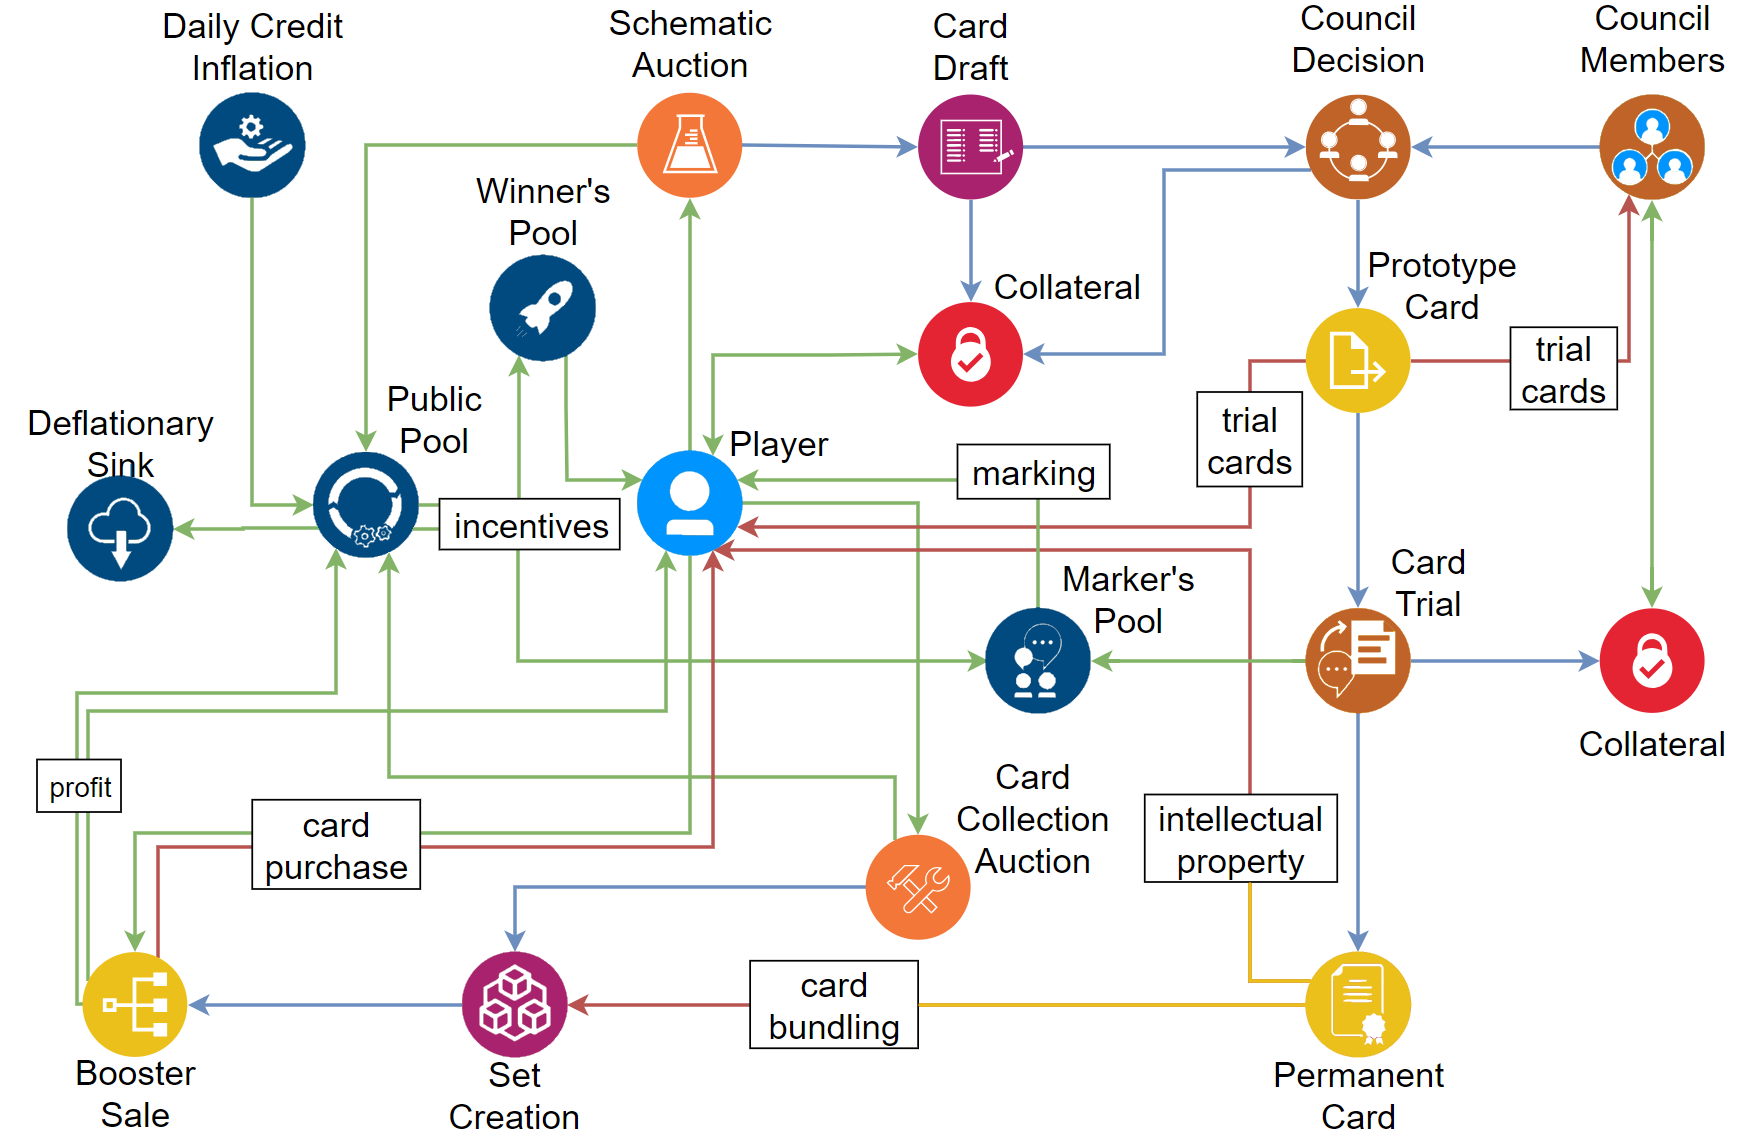
\includegraphics[width=1\textwidth]{flow.png}
	\caption{Here the flow of credits, cards and information is depicted. \textcolor{boringgreen}{Green} lines indicate credit flow, \textcolor{boringred}{cinder red} lines indicate card transfers and \textcolor{boringblue}{blue} lines processing of information. The circles indicate actors and processes. The \textcolor{awesomeblue}{blue} circles indicate global credit pools, sources and sinks, The \textcolor{awesomered}{red} circles indicate collateral credits locked up for some time, the \textcolor{awesomeorange}{orange} circles represent actions where users acquire the opportunity to create content, the \textcolor{awesomewinered}{winered} circles display processes where users create content, the \textcolor{awesomebrown}{brown} circles show where players judge cards, \textcolor{awesomeyellow}{yellow} indicates processes, where cards are created and \textcolor{awesomeskyblue}{sky blue} shows the players.
	}
	\label{fig1}
\end{figure}
%
On figure \ref{fig1} a flow chart of all processes except for card and credit transfer between players is depicted. What we haven't explained yet is the Daily Credit Inflation and the public pool. The latter has been mentioned in the text sometimes and it has the sole purpose of accumulating public credits and distributing these to the Winner's Pool and the Marker's Pool, there might also be a Tournament Pool, which allows to set up tournament prizes. The Daily Inflation is to fund the Public Pool with credits, when the game is bootstrapped and not many boosters are sold. In this phase there are not many player's and the Winner's Pool cannot be filled up with credits from booster sale. Therefore Daily Credit Inflation is necessary to allow for bootstrapping the network. This will be a fixed amount, independent on the size of the game and should be irrelevant compared to the inflationary process of the booster sale once the game has many players. 
%
\newline\newline
%
The auction system has to be explained as well. Card creation schematics and card collection boxes are the only things to be auctioned. The auction follows the ideas of the dutch auction system, let's start with the schematic. The auction starts with double the price of the last auction and this price is halfed every 60 minutes. So if every hour an auction is done, the price stays the same. The lowering of the price is not done once every 60 minutes, but 60 times an hour so that after 60 steps the price arrives at the half of the beginning price. This means every step the price is adjusted to roughly 98.84\% of the last price. If nobody buys the schematic, the price keeps falling and falling until someone actually makes a purchase. The next auction starts off at a much lower price and if people keep buying in the first minutes the price increases until an equilibrium is reached with schematics sold once every hour. The same principle applies to the auctioning of card collection boxes, but 
%
\section{Technology}
%
\end{document}